\subsection{Slučaj upotrebe: Kreiranje izbora}

\subsubsection*{Kratak opis}
Administrator kreira nove izbore i definiše period njihovog održavanja.

\subsubsection*{Akteri}
\begin{itemize}
    \item \textbf{Administrator} -- unosi podatke o izborima i potvrđuje njihovo kreiranje.
\end{itemize}

\subsubsection*{Preduslovi}
\begin{itemize}
    \item Administrator je prijavljen u sistem.
    \item Administrator ima ovlašćenje za kreiranje izbora.
\end{itemize}

\subsubsection*{Postuslovi}
\begin{itemize}
    \item U sistemu su evidentirani novi izbori sa definisanim periodom glasanja.
    \item Izbori još nisu spremni za glasanje, jer je potrebno formirati birački spisak i izborne liste.
\end{itemize}

\subsubsection*{Osnovni tok}
\begin{enumerate}
    \item Administrator bira opciju \textbf{Kreiraj izbore}.
    \item Sistem prikazuje formular za unos podataka o izborima.
    \item Administrator unosi naziv izbora, datum i vreme početka i datum i vreme kraja glasanja.
    \item Administrator potvrđuje unos.
    \item Sistem proverava ispravnost unetih podataka.
    \item Sistem čuva nove izbore i prikazuje poruku o uspešnom kreiranju.
\end{enumerate}

\subsubsection*{Alternativni tokovi}
\begin{enumerate}[label=\textbf{A\arabic*.}]
    \item \textbf{Neispravni ili nepotpuni podaci.} Ako administrator nije popunio sva polja ili je datum kraja glasanja pre datuma početka, sistem prikazuje poruku o grešci i omogućava ispravku podataka. Tok se nastavlja od koraka 3 osnovnog toka.
    \item \textbf{Odustajanje od kreiranja.} Administrator može da odustane od kreiranja izbora pre potvrde unosa. U tom slučaju sistem ne čuva podatke i slučaj upotrebe se završava.
\end{enumerate}

\begin{figure}[H]
    \centering
    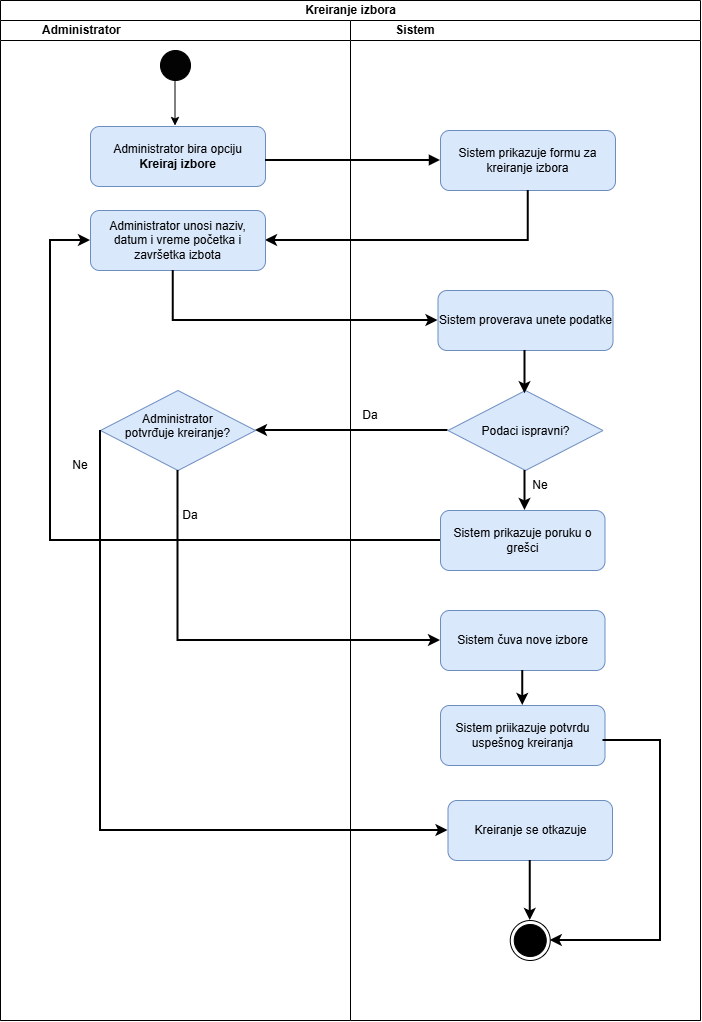
\includegraphics[width=0.8\textwidth]{kreiranje_izbora.png}
    \caption{Dijagram aktivnosti: Kreiranje izbora}
    \label{fig:kreiranje_izbora}
\end{figure}

\newpage
